\documentclass{beamer}
\mode<presentation>
\setbeameroption{show notes}

\usepackage{listings} % добавление листингов из исходников
\usepackage{IEEEtrantools} % для создания многострочных математических формул

\usepackage[utf8]{inputenc}
\usepackage[russian]{babel}
\usepackage{pdfpages}
\usepackage{graphicx}
\usepackage{tikz}
\usepackage{xcolor}
\usepackage{multirow}

\usepackage{amsfonts}

\setbeamertemplate{navigation symbols}{
	\insertframenavigationsymbol
	\raisebox{0.07cm}[0pt][0pt]{
    \insertframenumber/\inserttotalframenumber}
}

\setbeamertemplate{frametitle}[default][center]


\title{Local Alignment Kernels for Biological Sequences}
\author{Свичкарев Анатолий}

% поля титульного слайда
\institute{Санкт-Петербургский Государственный Политехнический Университет\\
    Петра Великого\\
    \vspace{0.7cm}
    Преподаватель:  к.н. Н.О. Кадырова\\
    \vspace{0.7cm}
}
\date{\today}

\begin{document}

% титульный слайд
\begin{frame}
\titlepage
\end{frame}

% \begin{frame}
% \frametitle{Вступление}
% \end{frame}

\begin{frame}
\frametitle{Локальное выравнивание последовательностей\\
Обозначения}
Выравнивание с пробелами:
\begin{equation*}
    \pi = ((\pi_1(1), \dots, \pi_1(p)),(\pi_2(1), \dots, \pi_2(p)))
    \in \mathbb{N}^{2p}
\end{equation*}

Пример: x = GAATCCG и y = GATTGC
\begin{equation*}
    \pi = ((1,2,4,6),(1,3,4,5))
\end{equation*}
\centerline{G-AATCCG-}\\
\centerline{GAT-T-G-C}
\end{frame}

\begin{frame}
\frametitle{Локальное выравнивание последовательностей\\
Алгоритм Смита-Ватермана}
Счёт локального выравнивания:
\begin{IEEEeqnarray*}{rCl}
    S_{S,g}(\pi)
    & = & \sum_{i=1}^{|\pi|}S(x_{\pi_1(i)}, y_{\pi_2(i)}) - \\
    - && \sum_{i=1}^{|\pi|-1}(g(\pi_1(i+1) - \pi_1(i))
    + g(\pi_2(i+1) - \pi_2(i)))
\end{IEEEeqnarray*}
Счёт Смита-Ватермана (SW):
\begin{equation*}
    SW_{S,g}(x, y) = \max_{\pi \in \Pi(x, y)} S_{S, g}(\pi)
\end{equation*}
\end{frame}


\begin{frame}
\frametitle{Подходит ли SW в качестве ядра?}
Напомим определение допустимого ядра:
\begin{itemize}
    \item симметрия:
    \begin{equation*}
        k(x, y) = k(y, x)
    \end{equation*}

    \item положительная полуопределённость:
    \begin{equation*}
        \forall n \in \mathbb{N},
        \forall (x_1, \dots, x_n, \alpha_1, \dots, \alpha_n)
            \in \chi^n \times \mathbb{R}^n:
    \end{equation*}
    \begin{equation*}
        \sum^n_{i, j = 1} \alpha_i \alpha_j k(x_i, x_j) \geq 0
    \end{equation*}
\end{itemize}
будем называть такие ядра \textit{\textbf{строковыми}}.

\bigskip
\textbf{Проблема:}\\
SW симметрично,\\но не всегда положительно полуопределено.

\bigskip
Авторы решили разобраться...
\end{frame}

\begin{frame}
\frametitle{Свёртка ядер}
Определение:

\begin{equation*}
    \sqsupset k_1, k_2 \mid k_i: \chi \times \chi \to \mathbb{R}.
\end{equation*}
Свёрткой $k_1$ и $k_2$
назовём $k_1 \star k_2$:
\begin{equation*}
    k_1 \star k_2(x, y)
    = \sum_{x_1 x_2 = x, y_1 y_2 = y} k_1(x_1, y_1) k_2(x_2, y_2)
\end{equation*}

\bigskip
Теорема:

Свёртка двух строковых ядер --- строковое ядро.
\end{frame}

\begin{frame}
    \frametitle{Построение ядра локального выравнивания (LA)}
    Сконструируем новое строковое ядро из трёх простых ядер.
    \bigskip

    Будем использовать:
    \begin{equation*}
        \forall (x, y) \in \chi^2
    \end{equation*}

    \begin{itemize}
        \item Края:
            \begin{equation*}
                k_0(x, y) = 1
            \end{equation*}

        \item Выровненные символы:
            \begin{equation*}
                k_\alpha^{(\beta)}(x, y) = \left\{ \,
                    \begin{IEEEeqnarraybox}[][c]{l?s}
                        \IEEEstrut
                        0 & если $|x| \ne 1$ или $|y| \ne 1$, \\
                        exp[\beta S(x, y)] & иначе.
                        \IEEEstrut
                    \end{IEEEeqnarraybox}
                    \right.
                    \label{eq:example_left_right1}
                \end{equation*}

        \item Пропуски:
            \begin{equation*}
                k_g^{(\beta)}(x, y) = exp[\beta (g(|x|) + g(|y|))]
            \end{equation*}
    \end{itemize}
\end{frame}

% \begin{frame}
% \frametitle{Ядро локального выравнивания}
% \end{frame}
%
% \begin{frame}
% \frametitle{Проблема диагонального преобладания}
% \end{frame}
%
% \begin{frame}
% \frametitle{Результаты эксперимента}
% \end{frame}

% \begin{frame}
% \frametitle{}
% \end{frame}
% подключения файла со слайдами

%!TEX root = svm.tex

\begin{frame}
\frametitle{Постановка задачи}	
	\begin{itemize}
		\item $X = \mathbb{R}^{n}$ - пространство объектов
		\item $Y = \{-1, +1\}$ - множество ответов
	\end{itemize}

	Задача обучения по $(x_i, y_i), x_i \in X, y_i \in Y$:
	\begin{equation*}
	\min_{w, b, \xi} \,\, \frac{1}{2} w^{T}w +  C \sum_{i = 1}^{l}\xi_{i}
	\end{equation*}
	При условии:
	\begin{equation*}
	y_{i}(w^{T} \phi(x_i) + b) \ge 1 - \xi{i}
	\end{equation*}
	\begin{equation*}
	\xi{i} \ge 0
	\end{equation*}

\end{frame}


\begin{frame}
\frametitle{Примеры ядер}
	\begin{itemize}
		\item Линейное: 
		\begin{equation*}
			K(x,y) = \langle x, y \rangle
		\end{equation*}

		\item Полиномиальное:
		\begin{equation*}
			K(x,y) = (\gamma \langle x, y \rangle + r)^2, \gamma > 0
		\end{equation*}

		\item Радиальная базисная функция (RBF):
		\begin{equation*}
			 K(x,y)= e^{-\gamma\left \| x - y \right \|^{2}}, \gamma > 0
		\end{equation*}

		\item Сигмоид:
		\begin{equation*}
			K(x,y) = \tanh(\gamma \langle x, y \rangle + r)
		\end{equation*}

	\end{itemize}
\end{frame}

\begin{frame}
\frametitle{Шаги обычного пользователя}
	\begin{enumerate}
		\item Преобразование данных к формату SVM пакета
		\item Произвольный выбор ядер и параметров алгоритма
		\item Тестирование
		\item Разочарование
	\end{enumerate}
\end{frame}


\begin{frame}
\frametitle{Шаги продвинутого пользователя}
	\begin{enumerate}
		\item Преобразование данных к формату SVM пакета
		\item \textbf{Масштабирование}
		\item \textbf{Рассмотрение радиальной базисной функции в роли ядра $K(x,y)= e^{-\gamma\left \| x - y \right \|^{2}}$}
		\item \textbf{С помощью кросс-валидации поиск наилучших $C$ и $\gamma$}
		\item \textbf{Дальнейшее обучение на всём множестве объектов}
		\item Тестирование
		\item \textbf{Счастье, радость}
	\end{enumerate}
\end{frame}


\begin{frame}
\frametitle{Преобразование к числовым параметрам}
	\begin{figure}[h]
		\center{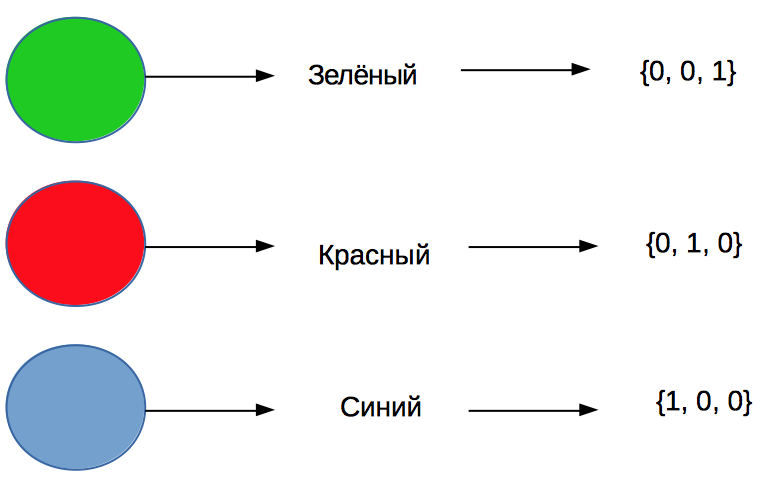
\includegraphics[width=\linewidth,height=7cm]{img/colors}}
	\end{figure}
\end{frame}


\begin{frame}
\frametitle{Масштабирование}
	\begin{itemize}
		\item Масштабируем в промежуток $[0, 1]$ или $[-1,+1]$
		\item Масштабируем как обучающуюся выборку, так и тестируемую выборку
		\item Решает проблему переполнения
	\end{itemize}
\end{frame}


\begin{frame}
\frametitle{Выбор радиального базисного ядра}
	\begin{itemize}
		\item Линейное и сигмоидное ядро схожи с радиальным базисным ядром
		\item Меньше количество параметров по сравнению с остальными ядрами
		\item Меньше проблем с переполнением
	\end{itemize}
\end{frame}


\begin{frame}
\frametitle{Кросс-валидация}

	\textbf{Кросс-валидация:}
	\begin{itemize}
		\item Разбиваем обучающуюся выборку произвольно на $n$ частей
		\item На $n - 1$ частях обучаемся, на оставшейся тестируем		
	\end{itemize}

	\textbf{Зачем?}
	\begin{itemize}
		\item Можем избежать проблем с переобучением
		\item Поиск оптимальных параметров $C$ и $\gamma$
	\end{itemize}
\end{frame}


\begin{frame}
\frametitle{Пример переобучения}
	\begin{figure}[h]
		\center{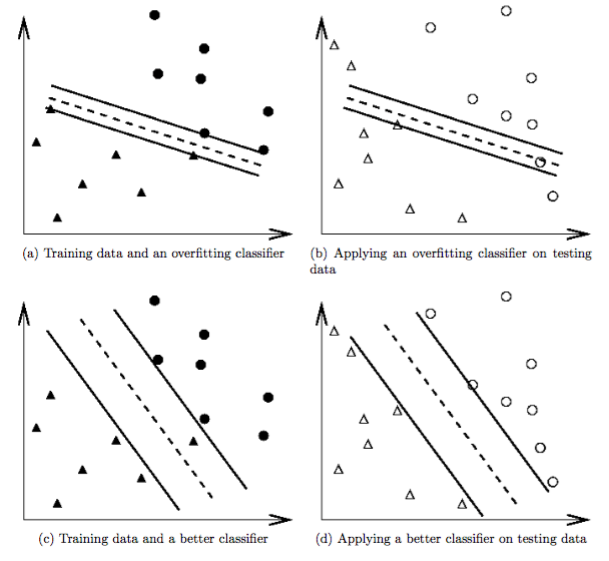
\includegraphics[width=\linewidth,height=7cm]{img/overfitting}}
	\end{figure}
\end{frame}

\begin{frame}
\frametitle{Сеточный поиск}
	\textbf{Поиск $C$ и $\gamma$:}
	\begin{itemize}
		\item Перебираем $C = 2^{-5}, 2^{-3},...,2^{15}$ и $\gamma = 2^{-15},2^{-13},...,2^{3}$
		\item Для каждой пары запускаем кросс-валидацию
		\item Определяем наилучшую пару
	\end{itemize}
	\textbf{Преимущества:}
	\begin{itemize}
		\item В силу независимости $C$ и $\gamma$ - легко распараллелить, в отличии от альтернативных методов
		\item Вычислительная сложность ненамного выше при аналогичных оптимизационных методах
		\item Эвристические методы не надёжны
	\end{itemize}
\end{frame}


\begin{frame}
\frametitle{LIBSVM}
	\textbf{Библиотека для поддержки SVM}
	\begin{itemize}
		\item Имеется интерфейс для R, MATLAB, Python, Haskell и т.д.
		\item Исходники на Java и C++
		\item Всевозможные настройки SVM
	\end{itemize}
\end{frame}

\begin{frame}
\frametitle{LIBSVM}
	\textbf{Интерфейс для командной строки:}
	\begin{itemize}
		\item \textbf{svm-scale} - мастштабирование
		\item \textbf{svm-train} - обучение
		\item \textbf{svm-predict} - предсказывание
	\end{itemize}
\end{frame}



\begin{frame}[fragile]
\frametitle{Примеры}
	\textbf{Обучаемся:}
	\begin{lstlisting}[language=bash]
	svm-train -v 5 svmguide2
	\end{lstlisting}
	Cross Validation Accuracy = 56.5217\%

	\textbf{Масштабируем:}
	\begin{lstlisting}[language=bash]
    svm-scale -l -1 -u 1 svmguide2 > svmguide2.s
    svm-train -v 5 svmguide2.s
	\end{lstlisting}
	Cross Validation Accuracy = 78.5166\%

	\textbf{Поиск оптимальных параметров:}
	\begin{lstlisting}[language=bash]
    python grid.py svmguide2.scale
	\end{lstlisting}
	Cross Validation Accuracy = 85.1662\%
\end{frame}





\begin{frame}[fragile]
\frametitle{Пример неправильного использования}

\begin{lstlisting}[language=bash]

svm-scale -l 0 svmguide4 > svmguide4.s
svm-scale -l 0 svmguide4.t > svmguide4.t.s
python easy.py svmguide4.s svmguide4.t.s
\end{lstlisting}
\textbf{Accuracy} = 69.2308\% (216/312) (classification)

\begin{lstlisting}[language=bash]
svm-scale -l 0 -s range4 svmguide4 > svmguide4.s
svm-scale -r range4 svmguide4.t > svmguide4.t.s
python easy.py svmguide4.s svmguide4.t.s
\end{lstlisting}
\textbf{Accuracy} = 89.4231\% (279/312) (classification)

\end{frame}



\begin{frame}[fragile]
\frametitle{LIBLINEAR vs LIBSVM}
	
	\textbf{LIBSVM:}
	\begin{lstlisting}[language=bash]
	time svm-train -c 4 -t 0 -e 0.1 -m 800 -v
	\end{lstlisting}
	Cross Validation Accuracy = 96.8136\%

	345.569s

	\textbf{LIBLINEAR}
	\begin{lstlisting}[language=bash]
	time train -c 4 -e 0.1 -v 5
	\end{lstlisting}

	Cross Validation Accuracy = 97.0161\%

	2.944s

\end{frame}

\end{document}
